\documentclass[12pt,answers]{exam}

\usepackage{tikz, pgfplots}
\usepackage{amsmath}
\usepackage{hyperref}
\usepackage[empty]{fullpage}

\newcounter{countA}


\begin{document}
\subsection*{Midterm 1 Suggested Review Problem Solutions}  

Here are problems that are similar to the ones you might see on the
exam. Be sure to also review old quiz and workshop questions too.

\subsubsection*{Data Basics}

Know all the terminology: Populations, Samples, Individuals (i.e., Observational Units), Variables, Statistics, Parameters, etc.


\begin{questions}
\setcounter{question}{\value{countA}}
\question (\href{http://people.hsc.edu/faculty-staff/blins/books/OpenIntroStats4e.pdf\#eoce.1.17}{Exercise 1.17 from OpenIntro Statistics}) The General Social Survey asked the question, ``After an average work day,
about how many hours do you have to relax or pursue activities that you enjoy?" to a random sample of 1,155
Americans. The average relaxing time was found to be 1.65 hours. Determine which of the following is an
observation, a variable, a sample statistic (value calculated based on the observed sample), or a population
parameter.
\begin{parts}
\part An American in the sample. 
\begin{solution}
Individual
\end{solution}
\bigskip

\part Number of hours spent relaxing after an average work day. 
\begin{solution}
Variable
\end{solution}
\bigskip

\part 1.65. 
\begin{solution}
Sample statistic
\end{solution}
\bigskip

\part Average number of hours all Americans spend relaxing after an average work day. 
\begin{solution}
Population parameter
\end{solution}
\bigskip
\end{parts}

\question (\href{http://people.hsc.edu/faculty-staff/blins/books/OpenIntroStats4e.pdf\#eoce.1.44}{Exercise 1.44 from OpenIntro Statistics}) The following summary table shows the number of space launches in the US by the
type of launching agency and the outcome of the launch (success or failure).
\begin{center}
\begin{tabular}{l|cc|cc}
\hline
& \multicolumn{2}{c|}{1957-1999} & \multicolumn{2}{|c}{2000-2018} \\ 
& Failure & Success & Failure & Success \\ \hline
Private & 13 & 295 & 10 & 562 \\
State & 281 & 3751 & 33 & 711 \\ 
Startup & - & - & 5 & 65 \\ \hline
\end{tabular}
\end{center}
\begin{parts}
\part What variables were collected on each launch in order to create to the summary table above?
\begin{solution}
There are three variables: the year, the launching agency, and the outcome. 
\end{solution}
\bigskip

\part State whether each variable is categorical or quantitative. 
\begin{solution}
The year is quantitative. The launching agency is categorical with three categories (private, state, or startup). The outcome is categorical with two categories (success or failure). 
\end{solution}
\part Suppose we wanted to study how the success rate of launches vary between launching agencies and over
time. In this analysis, which variable would be the response variable and which variable would be the
explanatory variable?
\begin{solution}
Both year and launching agency would be explanatory variables, and the outcome would be the response variable.  
\end{solution}
\bigskip

\end{parts}
\setcounter{countA}{\value{question}}
\end{questions}

\subsubsection*{Sampling}\label{sampling}

Make sure you know the difference between random error and bias. What is the best way to avoid bias?  What is the best way to minimize random error? 

\begin{questions}
\setcounter{question}{\value{countA}}
\question (\href{http://people.hsc.edu/faculty-staff/blins/books/OpenIntroStats4e.pdf\#eoce.1.26}{Exercise 1.26 from OpenIntro Statistics}) Suppose we want to estimate household size, where a ``household" is defined as people
living together in the same dwelling, and sharing living accommodations. If we select students at random
at an elementary school and ask them what their family size is, will this be a good measure of household
size? Or will our average be biased? If so, will it overestimate or underestimate the true value?
\begin{solution}
It will be biased because kids from larger families are more likely to be selected.  
\end{solution}
\bigskip

\question (\href{http://people.hsc.edu/faculty-staff/blins/books/OpenIntroStats4e.pdf\#eoce.1.39}{Exercise 1.39 from OpenIntro Statistics}) Identify the flaw(s) in reasoning in the following scenarios. Explain what the
individuals in the study should have done differently if they wanted to make such strong conclusions.
\begin{parts}
\part  Students at an elementary school are given a questionnaire that they are asked to return after their
parents have completed it. One of the questions asked is, ``Do you find that your work schedule makes
it difficult for you to spend time with your kids after school?" Of the parents who replied, 85\% said
``no". Based on these results, the school officials conclude that a great majority of the parents have no
difficulty spending time with their kids after school.
\begin{solution}
This is biased because parent's with more free time and who spend more time with their kids are more likely to fill out the questionnaire. A better approach might be to call a random sample of parents and ask them. 
\end{solution}
\bigskip


\part  A survey is conducted on a simple random sample of 1{,}000 women who recently gave birth, asking them
about whether or not they smoked during pregnancy. A follow-up survey asking if the children have
respiratory problems is conducted 3 years later. However, only 567 of these women are reached at the
same address. The researcher reports that these 567 women are representative of all mothers.
\begin{solution}
The women who moved might have moved for reasons that might be connected to whether their kids have respiratory problems.  For example, if there was mold in their houses.  It would be better to take a random sample of moms who currently have three year old children.
\end{solution}
\bigskip



\part An orthopedist administers a questionnaire to 30 of his patients who do not have any joint problems
and finds that 20 of them regularly go running. He concludes that running decreases the risk of joint
problems.
\begin{solution}
If the orthopedist is only looking at patients who don't have joint problems, then it is hard to compare whether running helps or hurts joints.  
\end{solution}
\bigskip



\end{parts}
\setcounter{countA}{\value{question}}
\end{questions}

\subsubsection*{Examining Numerical Data}

Make sure you know all of the different ways to plot a quantitative variable: Boxplots, Stemplots, Histograms. There will also be questions about how we measure the shape, center, and spread of a quantitative variable.

\begin{questions}
\setcounter{question}{\value{countA}}

\question (\href{http://people.hsc.edu/faculty-staff/blins/books/OpenIntroStats4e.pdf\#eoce.2.28}{Exercise 2.28(b) from OpenIntro Statistics}) The infant mortality rate is defined as the number of infant deaths per 1{,}000 live
births. This rate is often used as an indicator of the level of health in a country. The relative frequency
histogram below shows the distribution of estimated infant death rates for 224 countries for which such data
were available in 2014. Would you expect the mean of this data set
to be smaller or larger than the median?
Explain your reasoning.
\begin{flushright}
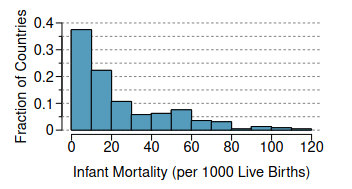
\includegraphics[scale=0.6]{infantMortality.png}
\end{flushright}
\begin{solution}
This data is skewed right so the mean will be greater than the median.
\end{solution}
\bigskip

\question (\href{http://people.hsc.edu/faculty-staff/blins/books/OpenIntroStats4e.pdf\#eoce.2.33}{Exercise 2.33 from OpenIntro Statistics}) Below are the final exam scores of twenty introductory statistics students.
$$57,~66,~69,~71,~72,~73,~74,~77,~78,~78,$$
$$79,~79,~81,~81,~82,~83,~83,~88,~89,~94$$
Create a box plot of the distribution of these scores.
\begin{solution}
The median is 78.5, $Q_1 = 72.5$, and $Q_3 = 82.5$.  Therefore the box plot is:

\begin{center}
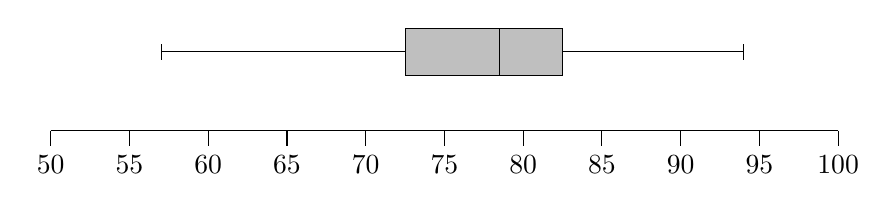
\begin{tikzpicture}
\draw (10,0) -- (20,0);
\foreach \x in {50,55,...,100} {
    \draw (\x / 5, 0) -- (\x /5, -0.2) node[below] {\x};
}
\draw[|-|] (11.4, 1) -- (18.8,1);
\filldraw[fill=gray!50] (14.5, 0.7) rectangle (16.5, 1.3);
\draw (15.7, 0.7) -- (15.7, 1.3);
\end{tikzpicture}
\end{center}

\end{solution}
\vspace*{2.5in}

\setcounter{countA}{\value{question}}
\end{questions}

\subsubsection*{Normal Distributions}

Make sure you comfortable with standardized values (z-values) and finding normal distribution proportions. Be sure to memorize the 68-95-99.7 rule.

\begin{questions}
\setcounter{question}{\value{countA}}

\question (\href{http://people.hsc.edu/faculty-staff/blins/books/OpenIntroStats4e.pdf\#eoce.4.4}{Exercise 4.4 from OpenIntro Statistics}) 
In triathlons, it is common for racers to be placed into age and gender groups.
Friends Leo and Mary both completed the Hermosa Beach Triathlon, where Leo competed in the Men, Ages
30 - 34 group while Mary competed in the Women, Ages 25 - 29 group. Leo completed the race in 1:22:28
(4948 seconds), while Mary completed the race in 1:31:53 (5513 seconds). Obviously Leo finished faster,
but they are curious about how they did within their respective groups. Can you help them? Here is some
information on the performance of their groups:
\begin{itemize}
\item The finishing times of the Men, Ages 30 - 34 group has a mean of 4313 seconds with a standard
deviation of 583 seconds.
\item The finishing times of the Women, Ages 25 - 29 group has a mean of 5261 seconds with a standard
deviation of 807 seconds.
\item The distributions of finishing times for both groups are approximately Normal.
\end{itemize}
Remember: a better performance corresponds to a faster finish.
\bigskip

\begin{parts}
\part Write down the short-hand for these two normal distributions.
\begin{solution}
Men 30 to 34 have a $N(4313, 583)$ distribution.  Women 25 to 29 have $N(5261, 807)$. 
\end{solution}
\bigskip

\part What are the Z-scores for Leo's and Mary's finishing times? What do these Z-scores tell you?
\begin{solution}
$z_\text{Leo} = \dfrac{4948 - 4313}{583} = 1.09$ and $z_\text{Mary} = \dfrac{5513 - 5261}{807} = 0.31$.
The z-scores tell you how many standard deviations Leo \& Mary were slower than average for their age groups. 
\end{solution}
\bigskip

\part Did Leo or Mary rank better in their respective groups? Explain your reasoning.
\begin{solution}
Mary ranks better since her z-score is lower which means she ran faster relative to her age group.
\end{solution}
\bigskip

\part What percent of the triathletes did Leo finish faster than in his group?
\begin{solution}
$$13.8\%$$
\end{solution}
\bigskip

\part What percent of the triathletes did Mary finish faster than in her group?
\begin{solution}
$$37.8\%$$
\end{solution}
\bigskip

\part If the distributions of finishing times are not nearly normal, would your answers to parts (b) - (e) change?
Explain your reasoning.
\begin{solution}
The answers for (d) \& (e) would not be trustworthy, because they came from the normal distribution app.
\end{solution}
\bigskip

\end{parts}

\vfill

\question (\href{http://people.hsc.edu/faculty-staff/blins/books/OpenIntroStats4e.pdf\#eoce.4.8}{Exercise 4.8 from OpenIntro Statistics}) The Capital Asset Pricing Model (CAPM) is a financial model that assumes returns on a
portfolio are normally distributed. Suppose a portfolio has an average annual return of 14.7\% (i.e. an
average gain of 14.7\%) with a standard deviation of 33\%. A return of 0\% means the value of the portfolio
doesn’t change, a negative return means that the portfolio loses money, and a positive return means that
the portfolio gains money.
\begin{parts}
\part What percent of years does this portfolio lose money, i.e. have a return less than 0\%?
\begin{solution}
$$P(X < 0) = 32.8\%$$
\end{solution}
\bigskip

\part What is the cutoff for the highest 15\% of annual returns with this portfolio?
\begin{solution}
48.9\% returns would be in the top 15\% of all annual returns. 
\end{solution}
\bigskip
\end{parts}

\question (\href{http://people.hsc.edu/faculty-staff/blins/books/OpenIntroStats4e.pdf\#eoce.4.44}{Exercise 4.44 from OpenIntro Statistics}) Heights of 10 year olds, regardless of gender, closely follow a normal
distribution with mean 55 inches and standard deviation 6 inches.
\begin{parts}
\part What is the probability that a randomly chosen 10 year old is shorter than 48 inches?
\begin{solution}
$$12.2\%$$
\end{solution}
\bigskip

\part What is the probability that a randomly chosen 10 year old is between 60 and 65 inches?
\begin{solution}
$$15.5\%$$
\end{solution}
\bigskip

\part If the tallest 10\% of the class is considered ``very tall", what is the height cutoff for ``very tall"?
\begin{solution}
$$62.7 \text{ inches}$$
\end{solution}
\bigskip

\end{parts}
\setcounter{countA}{\value{question}}
\end{questions}

\subsubsection*{Scatterplots \& Regression}

Make sure you can explain the meaning and the units of the slope of the least squares regression line.

\begin{questions}
\setcounter{question}{\value{countA}}

\question (\href{http://people.hsc.edu/faculty-staff/blins/books/OpenIntroStats4e.pdf\#eoce.1.40}{Exercise 1.40 from OpenIntro Statistics}) The scatterplot below shows the relationship between per capita income (in thousands of dollars) and percent of population with a bachelor's degree in 3{,}143 counties in the US in 2010.

\begin{center}
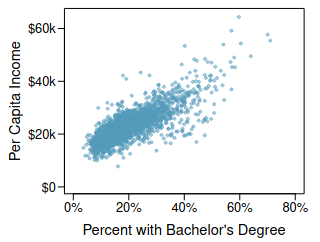
\includegraphics[scale=0.6]{percapitaIncome.png}
\end{center}

\begin{parts}
\item What are the explanatory and response variables?
\begin{solution}
Percent of population with bachelors degrees is explanatory and per capita income is response.
\end{solution}
\bigskip

\item Describe the relationship between the two variables. Make sure to discuss unusual observations, if any.
\begin{solution}
There is a moderately strong positive trend with no big outliers.
\end{solution}
\bigskip

\item Can we conclude that having a bachelor's degree increases one's income?
\begin{solution}
No, because correlation is not causation.
\end{solution}
\bigskip

\end{parts}

\question (\href{http://people.hsc.edu/faculty-staff/blins/books/OpenIntroStats4e.pdf\#eoce.8.8}{Exercise 8.8 from OpenIntro Statistics}) Match each correlation to the corresponding scatterplot.
\begin{center}
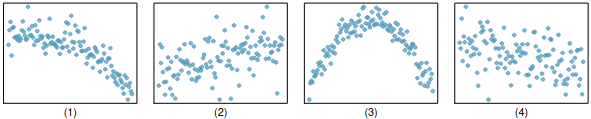
\includegraphics[scale=0.6]{correlations.png}
\end{center}

\begin{parts}
\part $R = 0.49$
\part $R = -0.48$
\part $R = -0.03$
\part $R = -0.85$
\end{parts}

\begin{solution}
(a) goes with (2), (b) goes with (4), (c) goes with (3), and (d) goes with (1).
\end{solution}
\bigskip

\setcounter{countA}{\value{question}}

\question (\href{http://people.hsc.edu/faculty-staff/blins/books/OpenIntroStats4e.pdf\#eoce.8.12}{Exercise 8.12 from OpenIntro Statistics}) A study conducted at the University of Denver investigated whether babies
take longer to learn to crawl in cold months, when they are often bundled in clothes that restrict their
movement, than in warmer months. Infants born during the study year were split into twelve groups, one
for each birth month. We consider the average crawling age of babies in each group against the average temperature when the babies are six months old (that’s when babies often begin trying to crawl). Temperature
is measured in degrees Fahrenheit ($^\circ$F) and age is measured in weeks.
\begin{center}
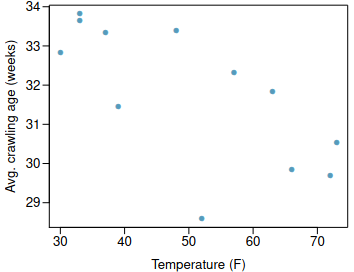
\includegraphics[scale=0.6]{babies.png}
\end{center}

\begin{parts}
\part Describe the relationship between
temperature and crawling age.
\begin{solution}
It is a moderate downward relationship.  It look like babies do learn to crawl sooner in warmer temperatures. 
\end{solution}
\bigskip


\part The correlation between temperature
in $^\circ$F and age in weeks was $r = -0.70$.
If we converted the temperature to $^\circ$C
and age to months, what would the
correlation be?
\begin{solution}
The correlation would not change.
\end{solution}
\bigskip
\end{parts}

\question (\href{http://people.hsc.edu/faculty-staff/blins/books/OpenIntroStats4e.pdf\#eoce.8.17}{Exercise 8.17 from OpenIntro Statistics}) Consider a regression predicting weight (kg) from height (cm) for a sample of
adult males. What are the units of the correlation coefficient, the intercept, and the slope?

\begin{solution}
The correlation coefficient doesn't have units.  The units for the y-intercept would be kilograms, and the slope would be measured in kilograms per centimeter. 
\end{solution}
\bigskip


\question (\href{http://people.hsc.edu/faculty-staff/blins/books/OpenIntroStats4e.pdf\#eoce.8.24}{Exercise 8.24 from OpenIntro Statistics}) Researchers studying anthropometry collected body girth measurements
and skeletal diameter measurements, as well as age, weight, height and gender for 507 physically active
individuals. The scatterplot below shows the relationship between height and shoulder girth (over deltoid
muscles), both measured in centimeters. 
\begin{center}
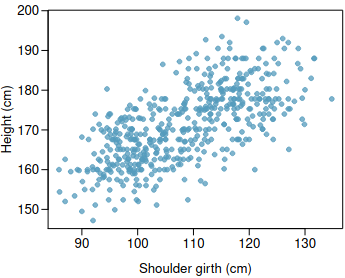
\includegraphics[scale=0.6]{girth.png}
\end{center}
The mean shoulder girth is 107.20 cm with a standard deviation of 10.37 cm. The mean
height is 171.14 cm with a standard deviation of 9.41 cm. The correlation between height and shoulder girth
is 0.67.
\begin{parts}
\item Write the equation of the regression line for predicting height.
\begin{solution}
$$y = 0.608 x + 106.0$$
\end{solution}
\bigskip

\item Interpret the slope in this context explain what it means using units.
\begin{solution}
The slope is 0.608 cm of height per cm of girth.  It means that for every extra cm of girth, you tend to be 0.608 cm taller.
\end{solution}
\bigskip

\item Calculate $R^2$ of the regression line for predicting height from shoulder girth, and interpret it in the context of the application.
\begin{solution}
$R^2 = 44.9\%$.  This means that 44.9\% of the variability in height follows the trend.  The remaining 55.1\% of the variability is above \& below the trend line.
\end{solution}
\bigskip

\item A randomly selected student from your class has a shoulder girth of 100 cm. Predict the height of this student using the model.
\begin{solution}
$$166.8 \text{ centimeters tall.}$$
\end{solution}
\bigskip

\item A one year old has a shoulder girth of 56 cm. Would it be appropriate to use this linear model to predict the height of this child?
\begin{solution}
No, that would be extrapolating past the data we have. 
\end{solution}
\bigskip

\end{parts}

\end{questions}

\end{document}
